% =======================================================================================================
% Artigo unificado: redes MLP sobre descritores de hits do MOMEA.
% Une (i) o estudo da bomba (MLP_EA_bomba.tex), (ii) o estudo na base CWRU (RELATORIO_CWRU.tex) e
% (iii) a inferência embarcada verificada por simulação (ARTIGO_SIM_EMBARCADO.tex).
% Figuras copiadas para figuras/; números da MicroBlaze em numeros_mb.tex (gerado por figuras_sim.py).
\documentclass[12pt]{article}
\usepackage[utf8]{inputenc}
\usepackage[T1]{fontenc}
\usepackage[brazilian]{babel}
\usepackage{amsmath, amssymb, amsfonts}
\usepackage{geometry}
\geometry{a4paper, margin=2.5cm}
\usepackage{graphicx}
\graphicspath{{figuras/}}
\usepackage[colorlinks=true, citecolor=blue, linkcolor=blue, urlcolor=blue]{hyperref}
\usepackage{xcolor}
\usepackage{array}
\usepackage{booktabs}
\usepackage{caption}
\usepackage{tikz}
\usetikzlibrary{arrows.meta, positioning}
\captionsetup{font=small, labelfont=bf}
\setlength{\parindent}{1.25cm}
\setlength{\emergencystretch}{3em}
\newcolumntype{L}[1]{>{\raggedright\arraybackslash}p{#1}}
\newcommand{\completar}[1]{\textcolor{red}{[#1]}}

% ---- números medidos na simulação RTL da MicroBlaze ----
% Gerado por embarcado/figuras_sim.py a partir de ciclos_mb.csv e dos ELFs. NÃO EDITAR.
\newcommand{\mbMlpIntSoftUs}{2\,053}
\newcommand{\mbMlpIntFpuUs}{1\,463}
\newcommand{\mbHitSoft}{38\,287}
\newcommand{\mbHitFpu}{4\,232}
\newcommand{\mbCargaEnsaioMax}{1}
\newcommand{\mbMlpFloatSoft}{3\,353\,499}
\newcommand{\mbMlpFloatFpu}{212\,130}
\newcommand{\mbQuantSoft}{66\,296}
\newcommand{\mbQuantFpu}{7\,232}
\newcommand{\mbMlpIntSoft}{139\,042}
\newcommand{\mbMlpIntFpu}{139\,042}
\newcommand{\mbHitHistSoft}{45\,323}
\newcommand{\mbHitHistFpu}{5\,122}
\newcommand{\mbFecharSoft}{749\,938}
\newcommand{\mbFecharFpu}{117\,676}
\newcommand{\mbFecharHistSoft}{214\,316}
\newcommand{\mbFecharHistFpu}{91\,974}
\newcommand{\mbParagrafoMlp}{Sem FPU, a inferência em float32 custou 3\,353\,499 ciclos (33{,}5\,ms), 16 vezes a inferência int8, porque cada operação de ponto flutuante é emulada em software. Com FPU, o float32 caiu para 212\,130 ciclos, 1{,}5 vezes o int8. O núcleo int8 não usa ponto flutuante e custou exatamente o mesmo nas duas configurações (139\,042 ciclos, ou 15{,}5 ciclos por multiplicação-acumulação dos 8\,960 pesos); a diferença entre elas está na quantização da entrada, com algumas dezenas de operações de ponto flutuante, que custou 66\,296 ciclos sem FPU e 7\,232 com FPU.}
\newcommand{\mbParagrafoCarga}{O custo por \textit{hit} é dominado pelos logaritmos, emulados em software sem FPU: 38\,287 ciclos sem FPU e 4\,232 com FPU, no modo exato. O histograma custa um pouco mais por \textit{hit} (45\,323 e 5\,122 ciclos), porque calcula o índice da classe, mas fecha a janela mais depressa (214\,316 contra 749\,938 ciclos sem FPU), porque não ordena: sem FPU, cada comparação da ordenação é uma chamada à biblioteca de ponto flutuante. Na taxa dos ensaios, cerca de 16 \textit{hits}/s nos dois canais, a cadeia completa ocupa 0{,}80\,\% da CPU sem FPU e 0{,}12\,\% com FPU. A 333 \textit{hits}/s por canal (666 no total), a ocupação chega a 25{,}7\,\% sem FPU e 2{,}9\,\% com FPU; nesse regime, a FPU passa a ser recomendável, ou o cálculo dos logaritmos por tabela.}
\newcommand{\mbTextoMin}{36{,}2}
\newcommand{\mbTextoMax}{42{,}4}
\newcommand{\mbTextoExatoSoft}{42{,}0}
\newcommand{\mbTextoExatoFpu}{36{,}2}
\newcommand{\mbTextoHistSoft}{42{,}4}
\newcommand{\mbTextoHistFpu}{36{,}7}
\newcommand{\mbParagrafoRota}{Na MicroBlaze sem FPU, a inferência int8 leva 2\,053\,\(\mu\)s, 0{,}041\,\% de uma janela, e mesmo o float32 emulado (33{,}5\,ms) seria aceitável; a rota em software não exige nenhum recurso adicional de lógica.}
\newcommand{\mbFatorHls}{18}


% =======================================================================================================
\title{\textbf{Diagnóstico de falhas na borda: classificação por MLP de descritores de emissão acústica extraídos em FPGA}}
\date{\today}
\author{Autores \\ Instituições \\ \texttt{email oficial}}
% =======================================================================================================
\begin{document}
\maketitle

\begin{abstract}
Este artigo avalia, de ponta a ponta, o uso de redes perceptron multicamadas (MLP) sobre descritores de \textit{hits} de emissão acústica (EA) extraídos na lógica programável do sistema MOMEA, desde o reconhecimento de condições de operação até a inferência no próprio FPGA. Em um ensaio de bomba com 56 corridas (8 frequências do motor \(\times\) 7 configurações das válvulas de recalque e sucção), os \textit{hits} foram agregados em 3\,540 janelas de 5\,s com 36 descritores, e uma MLP foi comparada a florestas aleatórias (RF) e \textit{gradient boosting} (GB) sob três validações sem sorteio de \textit{hits}. A frequência do motor generalizou para corridas e sessões não vistas (erro absoluto médio de 4,2 a 5,6\,Hz; 92 a 95\,\% das janelas a até \(\pm 10\)\,Hz), mas a configuração das válvulas caiu de 89--95\,\% de acurácia, com a corrida no treino, para 21--28\,\% (acaso: 14\,\%) com a corrida deixada de fora. Para separar limitações do método e dos dados, o mesmo fluxo foi aplicado à base pública de rolamentos da Case Western Reserve University (CWRU): com janelas sorteadas, todos os grupos de descritores chegaram a 87--92\,\% em quatro classes, mas, com rolamentos nunca vistos, a MLP caiu para 21\,\% (descritores clássicos), 25\,\% (\textit{hits} com limiar fixo), 46\,\% (\textit{hits} com limiar flutuante) e 63\,\% (envelope). Por fim, a cadeia de descritores e as duas MLPs foram portadas para o FPGA Artix-7 do MOMEA, quantizadas em int8 e verificadas em seis níveis de simulação: a cadeia em C reproduziu o modelo de referência em 100\,\% das janelas, o núcleo em síntese de alto nível ocupou 656 LUTs e 14 DSPs com 114\,\(\mu\)s por inferência, e a MicroBlaze simulada em RTL executou a inferência em \mbMlpIntFpuUs\ a \mbMlpIntSoftUs\,\(\mu\)s, com menos de \mbCargaEnsaioMax\,\% de CPU na taxa dos ensaios. Os resultados mostram que a MLP é viável na borda, mas que a capacidade de generalização depende sobretudo da validação por unidade física, da qualidade da aquisição e do limiar do extrator.
\end{abstract}

% =======================================================================================================
\section{Introdução}
\label{sec:introducao}

A emissão acústica é uma técnica passiva, adequada ao monitoramento contínuo de máquinas rotativas e hidráulicas. Colapsos de cavidades, turbulência do escoamento e impactos em defeitos localizados produzem ondas elásticas que se acoplam à carcaça e podem ser captadas por sensores externos \cite{brennen1995,neill1997,mba2006}. O MOMEA reduz o fluxo de amostras a registros de \textit{hits} parametrizados no FPGA --- amplitude de pico, contagens, tempo de subida, duração e energia --- à semelhança de instrumentos comerciais como o Vallen AMSY-6 \cite{unnthorsson2013,vallen2022}. A pergunta deste trabalho é prática: esses descritores bastam para que uma rede MLP reconheça o estado de uma máquina, com que confiança o resultado se generaliza e a que custo a inferência pode ser feita no próprio FPGA?

Três estudos, antes separados, compõem a resposta. O primeiro classifica as condições de operação de uma bomba a partir de \textit{hits} gravados pelo MOMEA. O segundo aplica o mesmo fluxo à base de rolamentos da CWRU \cite{cwru}, em que os defeitos são conhecidos e as unidades físicas são identificáveis, para distinguir o que é limitação do método do que é limitação dos dados da bomba. O terceiro leva o cálculo dos descritores e a MLP para o FPGA, em int8, e verifica a implementação por simulação, sem acesso às placas.

O fio condutor é a validação. \textit{Hits} e janelas de uma mesma corrida, ou de um mesmo rolamento, são fortemente correlacionados; sorteá-los entre treino e teste mede, em grande parte, a capacidade de reconhecer a corrida, e não a condição \cite{kaufman2012,roberts2017}. As contribuições são:
\begin{itemize}
	\item a comparação de MLP, RF e GB em descritores de \textit{hits} sob validações com independência crescente, na bomba e na CWRU (Seções~\ref{sec:metodos} e~\ref{sec:resultados});
	\item a demonstração, na CWRU, de que o limiar fixo do extrator falha diante de emissão contínua e de que um limiar flutuante recupera a periodicidade dos defeitos (Seção~\ref{subsec:res_cwru});
	\item a implementação embarcada da MLP int8 no Artix-7, em MicroBlaze e em lógica dedicada, verificada em seis níveis até a simulação RTL do processador (Seção~\ref{subsec:res_embarcado});
	\item uma discussão integrada das lições e recomendações para o MOMEA e para os próximos ensaios (Seção~\ref{sec:discussao}).
\end{itemize}

% =======================================================================================================
\section{Revisão bibliográfica}
\label{sec:revisao}

\subsection{Emissão acústica em máquinas e análise baseada em \textit{hits}}
\label{subsec:rev_ea}

O colapso de cavidades produz pulsos de pressão curtos e de banda larga, que excitam a estrutura numa faixa ampla de frequências \cite{brennen1995}. Em bombas centrífugas, a EA detectou a cavitação incipiente antes da queda mensurável de altura manométrica \cite{neill1997} e identificou o ponto de melhor eficiência de uma bomba de 60\,kW \cite{alfayez2005}. Combinando EA, vibração e visualização, \cite{mousmoulis2019} observaram que o nível de EA cresce com as primeiras bolhas, mas diminui em números de cavitação intermediários; a relação entre nível e severidade não é, portanto, monotônica. Em hidroturbinas, a cavitação foi monitorada pelo RMS da EA \cite{derakhshan1991}, e a detecção depende do tipo de cavitação e da posição do sensor \cite{escaler2006}. Revisões apontam a EA como eficaz na detecção precoce em rolamentos, bombas e engrenagens, mas sensível ao ruído de fundo e à atenuação \cite{mba2006,liu2023}.

A EA pode ser analisada pela forma de onda completa ou por parâmetros de cada \textit{hit} \cite{grosse2022}. A análise paramétrica reduz drasticamente o volume de dados, mas descarta a forma de onda e torna os descritores dependentes do limiar e dos parâmetros temporais (HDT, HLT, duração máxima) \cite{unnthorsson2013}; métodos de detecção distintos produzem inícios e términos diferentes para o mesmo sinal \cite{pinal2019}. Para emissão quase contínua, como a da cavitação desenvolvida, os \textit{hits} fundem-se ou atingem a duração máxima, e descritores de nível, como RMS e energia por intervalo, tendem a ser mais representativos \cite{derakhshan1991}. Sistemas comerciais mitigam o problema com limiar flutuante, que acompanha o nível de fundo \cite{vallen2022}.

\subsection{Diagnóstico de falhas por aprendizado de máquina e a base CWRU}
\label{subsec:rev_diagnostico}

O diagnóstico de falhas por aprendizado de máquina evoluiu de descritores manuais com classificadores rasos para redes profundas sobre o sinal bruto \cite{lei2020}. Um marco inicial é o uso de MLPs com descritores estatísticos no domínio do tempo (RMS, curtose, fator de crista) para rolamentos \cite{samanta2003}. Em rolamentos, o diagnóstico clássico baseia-se no espectro do envelope, que evidencia as frequências características de defeito \cite{randall2011}. A base CWRU \cite{cwru} tornou-se a referência para comparar métodos, e redes convolucionais sobre o sinal bruto relatam acurácias próximas de 100\,\%, inclusive sob ruído e mudança de carga \cite{zhang2017,zhang2018}.

Esses números, porém, dependem de como a base é dividida. O estudo de referência de \cite{smith2015} mostrou que parte das gravações é atípica e que os defeitos de esfera são de difícil diagnóstico mesmo com métodos clássicos. \cite{rauber2021} demonstraram que, quando janelas de uma mesma gravação estão no treino e no teste, a acurácia é inflada, e propuseram divisões que respeitam as gravações; \cite{hendriks2022} recomendaram separar os rolamentos físicos, já que cada rolamento com defeito foi gravado em quatro cargas. Em aplicações acústicas, \cite{amini2022} observaram que um classificador de cavitação treinado em pontos estáticos de uma hidroturbina falhou em ensaios dinâmicos, o que ilustra a mesma dificuldade de generalizar para condições não vistas.

\subsection{Modelos supervisionados: MLP, florestas aleatórias e \textit{gradient boosting}}
\label{subsec:rev_modelos}

A MLP compõe camadas de neurônios com ativação não linear e é treinada por retropropagação do gradiente do erro \cite{rumelhart1986}; com uma camada oculta suficientemente larga, aproxima qualquer função contínua num domínio compacto \cite{hornik1989}. Seu desempenho depende da padronização das entradas, do otimizador, tipicamente o Adam \cite{kingma2015}, da regularização e da parada antecipada \cite{prechelt1998}, cujo conjunto de validação define o que a rede aprende a generalizar. Para a borda, a MLP tem uma vantagem prática: sua inferência é uma sequência fixa de multiplicações e acumulações, adequada a FPGAs e à aritmética inteira \cite{duarte2018,jacob2018}.

A floresta aleatória (RF) combina centenas de árvores de decisão, cada uma treinada numa amostra \textit{bootstrap} e com um subconjunto aleatório de descritores em cada divisão; a média reduz a variância de uma árvore isolada, e o modelo é pouco sensível a hiperparâmetros \cite{breiman2001}. O \textit{gradient boosting} (GB) constrói as árvores sequencialmente, cada uma ajustada ao gradiente negativo da perda em relação às previsões acumuladas, numa descida de gradiente no espaço de funções \cite{friedman2001}; implementações como XGBoost \cite{chen2016} e LightGBM \cite{ke2017} acrescentam regularização e histogramas de descritores.

Em comparações amplas com dados tabulares, as florestas aleatórias estão entre os classificadores de melhor desempenho médio \cite{fernandezdelgado2014}, e modelos baseados em árvores igualam ou superam redes neurais com menor esforço de ajuste, em parte por serem robustos a descritores pouco informativos \cite{grinsztajn2022,shwartzziv2022}. Comparar as três famílias é, portanto, informativo: desempenhos semelhantes indicam que o limite está nos dados, e não no modelo.

\subsection{Validação com dados dependentes}
\label{subsec:rev_validacao}

Em dados com estrutura temporal ou hierárquica, como janelas de uma mesma corrida, a validação cruzada aleatória vaza informação entre treino e teste e superestima o desempenho; a recomendação é dividir por blocos que respeitem a estrutura de dependência \cite{kaufman2012,roberts2017}. A seleção de hiperparâmetros sobre o próprio teste introduz viés adicional, e a validação aninhada tem pouca resolução com poucas unidades independentes \cite{varma2006}.

\subsection{Inferência embarcada e quantização}
\label{subsec:rev_embarcado}

Os FPGAs permitem processar, em tempo real, EA amostrada a vários MSa/s \cite{kang2015,wirtz2018}, e ferramentas de síntese de alto nível (HLS) traduzem redes neurais em lógica com latências de microssegundos \cite{duarte2018,amd_ug1399}. A inferência inteira representa pesos e ativações em 8 bits com fatores de escala, acumula em 32 bits e requantiza por multiplicação inteira e deslocamento \cite{jacob2018,krishnamoorthi2018}; a quantização após o treino costuma custar pouca exatidão em redes pequenas, desde que as escalas sejam calibradas em dados representativos \cite{nagel2021}. Os trabalhos citados concentram-se numa aplicação específica e não verificam, bit a bit, a fidelidade da cadeia completa de descritores e inferência ao modelo de referência.

% =======================================================================================================
\section{Materiais e métodos}
\label{sec:metodos}

\subsection{Extração de \textit{hits} no MOMEA}
\label{subsec:extrator}

O extrator do MOMEA opera sobre o sinal retificado: o \textit{hit} começa no primeiro cruzamento do limiar e termina após HDT sem cruzamentos; segue-se um bloqueio re-armável (HLT), em que um cruzamento reinicia a espera e marca o próximo \textit{hit} com o indicador ROVL; \textit{hits} mais longos que a duração máxima são truncados e marcados com MAXDUR. Cada registro de 32 bytes traz amplitude de pico, contagens, tempo de subida, duração e energia bruta \(\sum u^2\), enviados por UDP ao computador.

\subsection{Ensaio da bomba}
\label{subsec:bomba}

A bancada \completar{descrever: bomba, motor e inversor, tubulação, sensores de EA e posição dos canais A e B} foi operada em delineamento cruzado: oito frequências do motor (20 a 90\,Hz, em passos de 10\,Hz) combinadas com sete configurações de abertura das válvulas de recalque e sucção (100-100, 100-75, 100-50, 100-25, 75-100, 50-100 e 25-100). Cada combinação foi registrada uma única vez, por cerca de 300\,s, num total de 56 corridas e 283\,618 \textit{hits} em dois canais, com ganho de 34\,dB, HDT de \(250\,\mu\)s, HLT de 2\,ms e duração máxima de 100\,ms. Cada série de válvulas foi ensaiada em bloco contínuo, ao longo de dois dias, com limiares diferentes entre sessões (Tabela~\ref{tab:ordem}); as válvulas estão, portanto, confundidas com o dia, o horário e o limiar.

\begin{table}[!htbp]
	\centering
	\caption{Séries de válvulas, horários, sentido da varredura de frequência e limiares.}
	\label{tab:ordem}
	\small
	\begin{tabular}{llll}
		\toprule
		\textbf{Série} & \textbf{Dia e horário} & \textbf{Ordem das freq.} & \textbf{Limiar A/B (dB\(_{\mathrm{AE}}\))} \\
		\midrule
		100-100 & 05/11, 10h42--12h09 & 30\(\rightarrow\)90, depois 20 & 63/50 (20\,Hz: 65/55) \\
		25-100 & 05/11, 15h54--16h41 & 90\(\rightarrow\)20 & 65/55 \\
		100-50 & 05/11, 16h52--17h45 & 90\(\rightarrow\)20 & 65/55 \\
		100-25 & 06/11, 09h49--10h32 & 20\(\rightarrow\)90 & 50/50 \\
		100-75 & 06/11, 11h17--12h01 & 20\(\rightarrow\)90 & 50/50 \\
		75-100 & 06/11, 14h49--15h32 & 20\(\rightarrow\)90 & 50/50 \\
		50-100 & 06/11, 15h52--16h41 & 20\(\rightarrow\)90 & 50/50 \\
		\bottomrule
	\end{tabular}
\end{table}

A inspeção dos registros revelou quatro problemas que condicionam a análise. (i) \textbf{Saturação}: 69,8\,\% dos \textit{hits} atingiram o fundo de escala do conversor (102,0 a 102,8\,dB\(_{\mathrm{AE}}\) referidos ao sensor), praticamente todos a partir de 40 a 50\,Hz (Figura~\ref{fig:exemplo}). (ii) \textbf{Duração máxima}: 17,8\,\% dos \textit{hits}, quase todos do canal A, foram truncados em 100\,ms, o que indica emissão contínua. (iii) \textbf{Cadência imposta pelo rearme}: o ROVL está ativo em 100\,\% dos \textit{hits}, e cada canal registra cerca de 10 \textit{hits}/s em quase todas as condições, de modo que a taxa de \textit{hits} não mede a atividade acústica. (iv) \textbf{Limiar variável} entre sessões, que afeta duração, contagens e energia sem correção posterior possível.

\begin{figure}[!htbp]
	\centering
	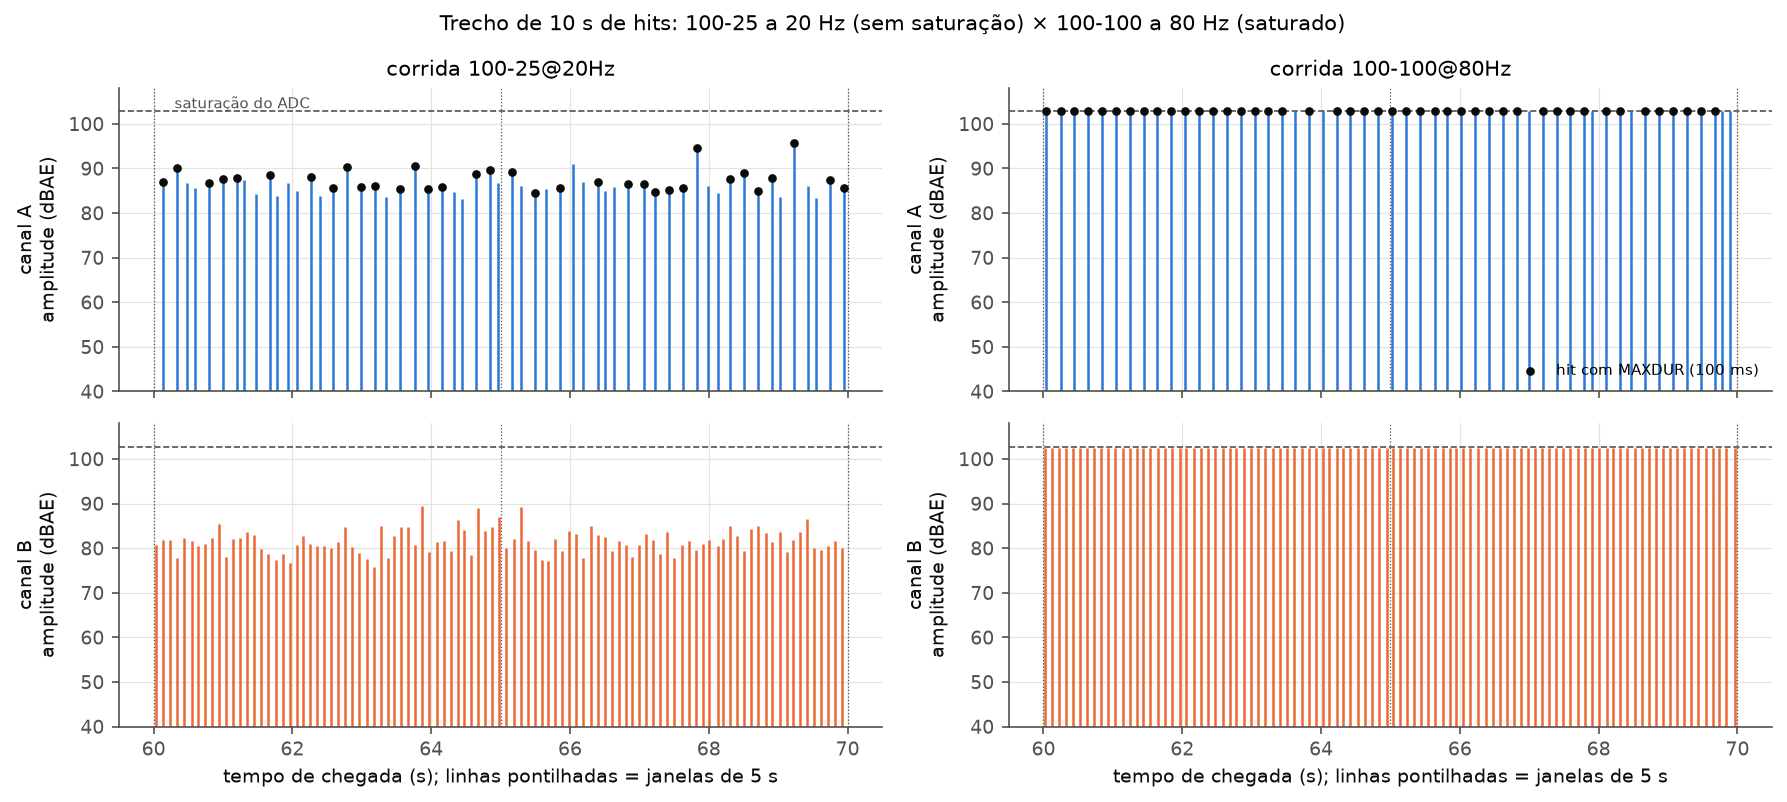
\includegraphics[width=0.92\textwidth]{fig_exemplo_hits.png}
	\caption{Trechos de 10\,s de \textit{hits} em duas corridas. A 20\,Hz (esquerda), as amplitudes variam e não há saturação. A 80\,Hz (direita), todos os \textit{hits} estão no fundo de escala e quase todos os do canal A atingem a duração máxima (pontos pretos). As linhas pontilhadas marcam as janelas de 5\,s.}
	\label{fig:exemplo}
\end{figure}

\paragraph{Descritores.} Como cavitação e ruído de escoamento são quase contínuos, os \textit{hits} foram agregados em janelas consecutivas de \(T_w = 5\)\,s, sem sobreposição: 3\,540 janelas, cerca de 63 por corrida. Por janela e canal calcularam-se 18 descritores (36 no total). Com todos os \textit{hits}: taxa, fração saturada, fração MAXDUR, frequência média mediana e o logaritmo da energia por segundo,
\begin{equation}
	E_s = \log_{10}\!\Big(\frac{1}{T_w}\sum_{i\in w} E_i + 1\Big),
	\label{eq:energia_s}
\end{equation}
que funciona como indicador de nível RMS. Só com os \textit{hits} sem MAXDUR: média e percentis 10, 50 e 90 da amplitude; percentis 50 e 90 de \(\log_{10}\) da energia, da duração e das contagens; e medianas do \(\log_{10}\) do tempo de subida, da frequência média e do \(\log_{10}\) de \(\mathrm{RA} = t_{\mathrm{sub}}/A_{\mathrm{pico}}\) \cite{ohno2010}. Valores faltantes (6,7\,\%) foram imputados pela mediana, e imputação e padronização foram ajustadas só no treino de cada partição.

\paragraph{Alvos.} A frequência do motor, ordenada, foi tratada como regressão, com leitura ordinal pelo arredondamento ao nível mais próximo. A configuração das válvulas foi modelada como uma classe de 7 níveis, equilibrada com 8 corridas por classe.

\subsection{Base CWRU}
\label{subsec:cwru}

Foram usados os sinais do acelerômetro do lado do acionamento, a 48\,kHz, dos conjuntos \textit{48k Drive End Bearing Fault Data} e \textit{Normal Baseline Data} \cite{cwru}. O rolamento 6205-2RS tem frequências de defeito iguais a 5,4152 (pista interna, BPFI), 3,5848 (pista externa, BPFO) e 2,3570 (esfera, BSF) vezes a rotação. O subconjunto tem delineamento cruzado completo: máquina sã (N) e defeitos por eletroerosão na pista interna (IR), na esfera (B) e na pista externa (OR@6h), com diâmetros de 0,007, 0,014 e 0,021~polegada, nas cargas de 0 a 3\,HP. São 40 gravações, divididas em 1\,376 janelas de 0,25\,s. Inconsistências conhecidas dos arquivos (variáveis de outras gravações, rotação ausente, amostras repetidas em \(\pm 3{,}418\,g\)) foram tratadas explicitamente.

Os sinais são de vibração, e não de EA; o extrator do MOMEA é aplicado como detector de impulsos, com os tempos escalados para 48\,kHz (HDT e HLT de 1\,ms; duração máxima de 20\,ms). Dois limiares foram comparados: \textbf{fixo}, de 0,3\,\(g\), como o MOMEA opera hoje; e \textbf{flutuante}, igual a 1,5 vez o RMS da janela anterior (causal), com mínimo de 0,3\,\(g\), análogo ao de sistemas comerciais \cite{vallen2022}. O fator 1,5 foi escolhido por varredura, pela concordância da ordem do intervalo entre \textit{hits} com BPFO e BPFI, o que usa os rótulos, mas não a divisão de treino e teste.

Três grupos de descritores foram calculados por janela: \textbf{clássicos} (8: RMS, pico, fator de crista, curtose, assimetria e fatores de forma, impulso e folga) \cite{samanta2003}; \textbf{envelope} (7: curtose do envelope e amplitudes do espectro do envelope em 1\(\times\) e 2\(\times\) BPFO, BPFI e 2\(\times\)BSF, com o sinal filtrado entre 1 e 10\,kHz) \cite{randall2011}; e \textbf{\textit{hits}} (14: taxa, frações truncadas e com ROVL, percentis de amplitude, energia, duração, contagens, subida e frequência média e, como descritores de periodicidade, a ordem do intervalo entre \textit{hits}, \((1/\mathrm{mediana}\,\Delta t)/f_r\), e seu coeficiente de variação). As tarefas foram quatro classes (N, IR, B, OR) e dez classes (tipo e diâmetro).

\subsection{Modelos}
\label{subsec:modelos}

Os modelos foram implementados no scikit-learn \cite{pedregosa2011}, com hiperparâmetros fixos, precedidos de imputação e padronização no mesmo \textit{pipeline}:
\begin{itemize}
	\item \textbf{MLP}: camadas ocultas de 64 e 32 neurônios, ReLU, Adam, penalidade L2 \(\alpha = 10^{-3}\) e parada antecipada com 15\,\% do treino como validação interna e paciência de 30 épocas \cite{prechelt1998}; na regressão, o alvo também é padronizado;
	\item \textbf{RF}: 300 árvores, mínimo de 2 amostras por folha e 50\,\% dos descritores por divisão na regressão (\(\sqrt{p}\) na classificação) \cite{breiman2001};
	\item \textbf{GB}: \textit{HistGradientBoosting}, com 300 iterações na regressão e 200 na classificação e taxa de aprendizado de 0,05 \cite{friedman2001} (apenas na bomba).
\end{itemize}
A ausência de busca de hiperparâmetros é deliberada: com 56 corridas, ou nove rolamentos com defeito, uma busca aninhada teria pouca resolução \cite{varma2006}. Os números são linhas de base.

\subsection{Validação}
\label{subsec:validacao}

Nenhuma validação da bomba sorteia \textit{hits} ou janelas. Foram usados três esquemas, com independência crescente \cite{roberts2017}:
\begin{description}
	\item[BLOCOS (5 partições):] cada corrida é dividida em 5 trechos consecutivos de cerca de 60\,s; o \(k\)-ésimo trecho de todas as corridas é o teste, com uma janela de exclusão de cada lado. A corrida aparece no treino e no teste.
	\item[LORO (\textit{leave-one-run-out}, 56 partições):] uma corrida inteira é o teste; sua frequência aparece no treino com outras válvulas e sua configuração com outras frequências.
	\item[LOSO (\textit{leave-one-series-out}, 7 partições, só frequência):] uma série de válvulas inteira, isto é, uma sessão contínua, é o teste.
\end{description}
Na CWRU, os esquemas foram: \textbf{janelas sorteadas} (5 partições estratificadas); \textbf{carga deixada de fora} (LOLO, 4 partições), que separa gravações mas não rolamentos; e \textbf{diâmetro deixado de fora} (3 partições, quatro classes), em que o teste contém rolamentos físicos nunca vistos, análogo ao LORO da bomba. As métricas são o erro absoluto médio (MAE), o \(R^2\) e o acerto do nível para a frequência, e a acurácia por janela e por corrida ou gravação (voto majoritário) para as classes.

\subsection{Implementação embarcada e verificação}
\label{subsec:embarcado}

A Figura~\ref{fig:cadeia} mostra a cadeia embarcada no XC7A35T do MOMEA. A MicroBlaze converte cada registro bruto em unidades físicas, acumula o \textit{hit} na janela corrente e, a cada 5\,s, calcula os 36 descritores, padroniza e quantiza a entrada e executa as duas redes de implantação (regressor 36-64-32-1 e classificador 36-64-32-7, cerca de 4,6 mil parâmetros cada, retreinados com todas as janelas). Os percentis são calculados em dois modos: \textbf{exato}, com vetores de até 1\,024 valores por canal ordenados por \textit{heapsort} (65,6\,kB), ou por \textbf{histograma} de largura fixa (10,3\,kB, independentemente da taxa de \textit{hits}).

\begin{figure}[!htbp]
	\centering
	\begin{tikzpicture}[
		font=\small, node distance=4mm and 4mm,
		bloco/.style={draw, rounded corners=2pt, align=center, minimum height=11mm, text width=22mm, fill=white},
		hw/.style={bloco, fill=blue!6},
		sw/.style={bloco, fill=orange!8},
		seta/.style={-{Latex[length=2mm]}, thick}]
		\node[hw] (det) {Detector de \textit{hits}\\(lógica do MOMEA)};
		\node[sw, right=of det] (conv) {Registro \(\to\)\\unidades físicas\\e limiar};
		\node[sw, right=of conv] (jan) {Janela de 5\,s:\\contagens, somas\\e percentis};
		\node[sw, right=of jan] (pre) {Imputação,\\padronização\\e int8};
		\node[hw, below=12mm of pre] (hls) {Núcleo int8\\(IP HLS)};
		\node[sw, left=of hls] (mbn) {Núcleo int8\\(C na MicroBlaze)};
		\node[bloco, left=of mbn, text width=30mm] (out) {Frequência (Hz)\\e classe de válvulas};
		\draw[seta] (det) -- node[above, font=\scriptsize]{32\,B} (conv);
		\draw[seta] (conv) -- (jan);
		\draw[seta] (jan) -- node[above, font=\scriptsize]{36} (pre);
		\draw[seta] (pre) -- (hls);
		\draw[seta] (pre.south west) to[out=-120, in=60] (mbn.north);
		\draw[seta] (mbn) -- (out);
		\draw[seta] (hls.south) to[out=-150, in=-30] (out.south);
	\end{tikzpicture}
	\caption{Cadeia embarcada. Em azul, lógica dedicada; em laranja, software na MicroBlaze. O núcleo int8 tem uma única fonte em C, que compila para a MicroBlaze ou é sintetizada como IP pelo Vitis HLS.}
	\label{fig:cadeia}
\end{figure}

As redes foram quantizadas após o treino, com pesos simétricos por camada e escalas de ativação calibradas no percentil 99,9. Uma camada densa com ReLU fica
\begin{equation}
	\begin{gathered}
	a_o = \sum_{i} q^{x}_{i}\, q^{W}_{io} + q^{b}_{o}, \qquad
	M = \mathrm{round}\!\left(2^{31}\,\frac{s_x\, s_W}{s_y}\right), \\
	q^{y}_{o} = \min\!\left(127,\ \left\lfloor \frac{\max(a_o, 0)\, M + 2^{30}}{2^{31}} \right\rfloor\right),
	\end{gathered}
	\label{eq:requant}
\end{equation}
em que \(s_x\), \(s_W\) e \(s_y\) são as escalas da entrada, dos pesos e da saída \cite{jacob2018,krishnamoorthi2018}. A Equação~\eqref{eq:requant} é determinística, o que permite exigir igualdade bit a bit; para isso, a quantização da entrada foi emulada em Python em precisão simples, com o mesmo arredondamento do C \cite{goldberg1991,ieee754}. Um único código-fonte do núcleo compila para o computador, para a MicroBlaze e para o Vitis HLS, este com \textit{pipeline} de intervalo 1 por laço interno e interface AXI4-Lite \cite{amd_ug1399}.

A verificação, feita sem acesso às placas, foi organizada em seis níveis: V0, a exportação do modelo; V1, a inferência em C nas 3\,540 janelas, em float32 e int8; V2, a cadeia completa a partir dos 281\,595 \textit{hits} brutos (após harmonizar o limiar); V3, a simulação C e a cossimulação C/RTL do núcleo HLS; V4, a síntese e o roteamento do IP no XC7A35T a 100\,MHz; e V5, a simulação RTL de um sistema MicroBlaze (Vivado 2022.2, memória local de 128\,kB, sem caches), executando o binário final, sem e com FPU, com ciclos medidos por marcas em GPIO \cite{amd_ug900,amd_ug984}. Na CWRU, a MLP de cada partição LOLO foi quantizada com a mesma aritmética, com escalas calibradas apenas no treino da partição.

% =======================================================================================================
\section{Resultados}
\label{sec:resultados}

\subsection{Bomba: frequência do motor}
\label{subsec:res_freq}

Com a corrida presente no treino (BLOCOS), o MAE da frequência ficou entre 1,1 e 2,1\,Hz (Tabela~\ref{tab:freq}). Com a corrida ou a série inteira fora do treino, subiu para 4,2 a 5,6\,Hz, mas 92 a 95\,\% das janelas continuaram a até um nível do valor real. Os níveis de 20 e 30\,Hz, sem saturação, são reconhecidos quase sempre; os erros concentram-se entre níveis vizinhos de 40 a 90\,Hz, onde a saturação achata a amplitude (Figura~\ref{fig:pr_loro}). RF e GB tiveram MAE menor, e a MLP acertou mais o nível exato em LORO (69\,\% contra 61\,\%); com 56 corridas, nenhuma diferença entre modelos é conclusiva. Em LOSO, o pior caso foi a série 100-25 (MAE de 9,9 a 10,6\,Hz), a mais distinta, com sucção estrangulada. As séries ensaiadas em ordem decrescente tiveram MAE de 3,6 a 7,9\,Hz, e um teste entre dias deu 4,0 a 6,6\,Hz: a previsão não se apoia apenas no sentido da varredura nem na sessão.

\begin{table}[!htbp]
	\centering
	\caption{Bomba, frequência do motor. MAE em Hz; Nível = acerto da previsão arredondada a 20, 30, \ldots, 90\,Hz; Corrida = acerto do nível pela mediana das janelas da corrida.}
	\label{tab:freq}
	\small
	\begin{tabular}{llrrrrr}
		\toprule
		\textbf{Validação} & \textbf{Modelo} & \textbf{MAE} & \(\boldsymbol{R^2}\) & \textbf{Nível} & \(\boldsymbol{\pm}\)\textbf{10\,Hz} & \textbf{Corrida} \\
		\midrule
		BLOCOS & MLP & 2,06 & 0,962 & 0,927 & 0,991 & 0,982 \\
		BLOCOS & RF & 1,08 & 0,985 & 0,943 & 0,990 & 0,982 \\
		BLOCOS & GB & 1,16 & 0,983 & 0,952 & 0,988 & 0,982 \\
		\midrule
		LORO & MLP & 5,61 & 0,790 & 0,691 & 0,918 & 0,714 \\
		LORO & RF & 4,85 & 0,883 & 0,612 & 0,942 & 0,589 \\
		LORO & GB & 4,97 & 0,879 & 0,608 & 0,949 & 0,625 \\
		\midrule
		LOSO & MLP & 5,09 & 0,850 & 0,698 & 0,939 & 0,768 \\
		LOSO & RF & 4,23 & 0,885 & 0,691 & 0,951 & 0,679 \\
		LOSO & GB & 4,21 & 0,888 & 0,701 & 0,951 & 0,714 \\
		\bottomrule
	\end{tabular}
\end{table}

\begin{figure}[!htbp]
	\centering
	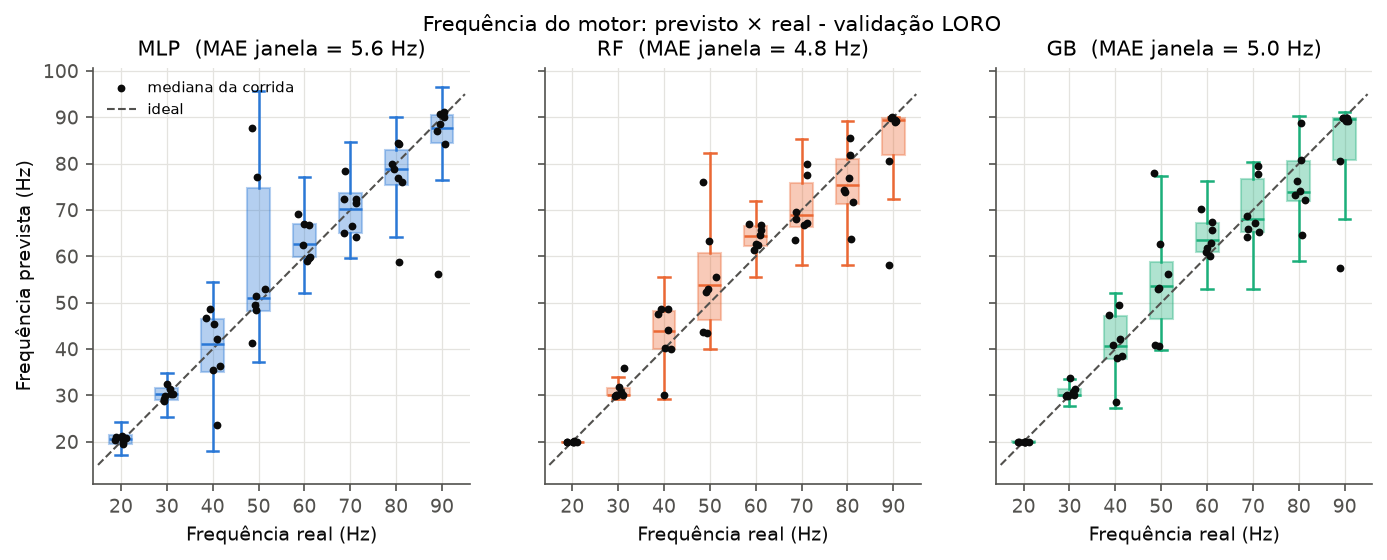
\includegraphics[width=0.85\textwidth]{fig_freq_previsto_real_LORO.png}
	\caption{Bomba: frequência prevista \(\times\) real com a corrida deixada de fora (LORO). Caixas: distribuição das janelas; pontos: mediana de cada corrida.}
	\label{fig:pr_loro}
\end{figure}

\subsection{Bomba: configuração das válvulas}
\label{subsec:res_valv}

A Tabela~\ref{tab:valv} e a Figura~\ref{fig:blocos_loro} mostram o contraste central do estudo da bomba. Em BLOCOS, as válvulas parecem bem reconhecidas: 89 a 95\,\% por janela e 100\,\% por corrida. Em LORO, a acurácia cai para 21 a 28\,\%, pouco acima do acaso de 14\,\%, e os acertos de \% recalque e \% sucção ficam no nível de um classificador que sempre responde 100\,\%. Os modelos aprendem, portanto, a assinatura de cada corrida --- acoplamento, deriva térmica, limiar da sessão --- e ela não se transfere para a mesma configuração em outra frequência. As confusões em LORO são sistemáticas (75-100 com 50-100; 100-75 e 100-50 com 100-25). Com uma corrida por condição, não é possível separar um efeito de válvula de um efeito de sessão.

\begin{table}[!htbp]
	\centering
	\caption{Bomba, configuração das válvulas (7 classes): acurácia por janela, F1 macro, acertos de \% recalque e \% sucção derivados da classe e acurácia por corrida (voto majoritário).}
	\label{tab:valv}
	\small
	\begin{tabular}{llrrrrr}
		\toprule
		\textbf{Validação} & \textbf{Modelo} & \textbf{Acurácia} & \textbf{F1} & \textbf{\% rec} & \textbf{\% suc} & \textbf{Corrida} \\
		\midrule
		BLOCOS & MLP & 0,888 & 0,888 & 0,919 & 0,946 & 1,000 \\
		BLOCOS & RF & 0,945 & 0,944 & 0,958 & 0,970 & 1,000 \\
		BLOCOS & GB & 0,934 & 0,933 & 0,948 & 0,964 & 1,000 \\
		\midrule
		LORO & MLP & 0,280 & 0,276 & 0,573 & 0,594 & 0,304 \\
		LORO & RF & 0,210 & 0,194 & 0,535 & 0,530 & 0,179 \\
		LORO & GB & 0,224 & 0,209 & 0,546 & 0,532 & 0,232 \\
		\midrule
		\multicolumn{2}{l}{Acaso} & 0,143 & --- & 0,571 & 0,571 & 0,143 \\
		\bottomrule
	\end{tabular}
\end{table}

\begin{figure}[!htbp]
	\centering
	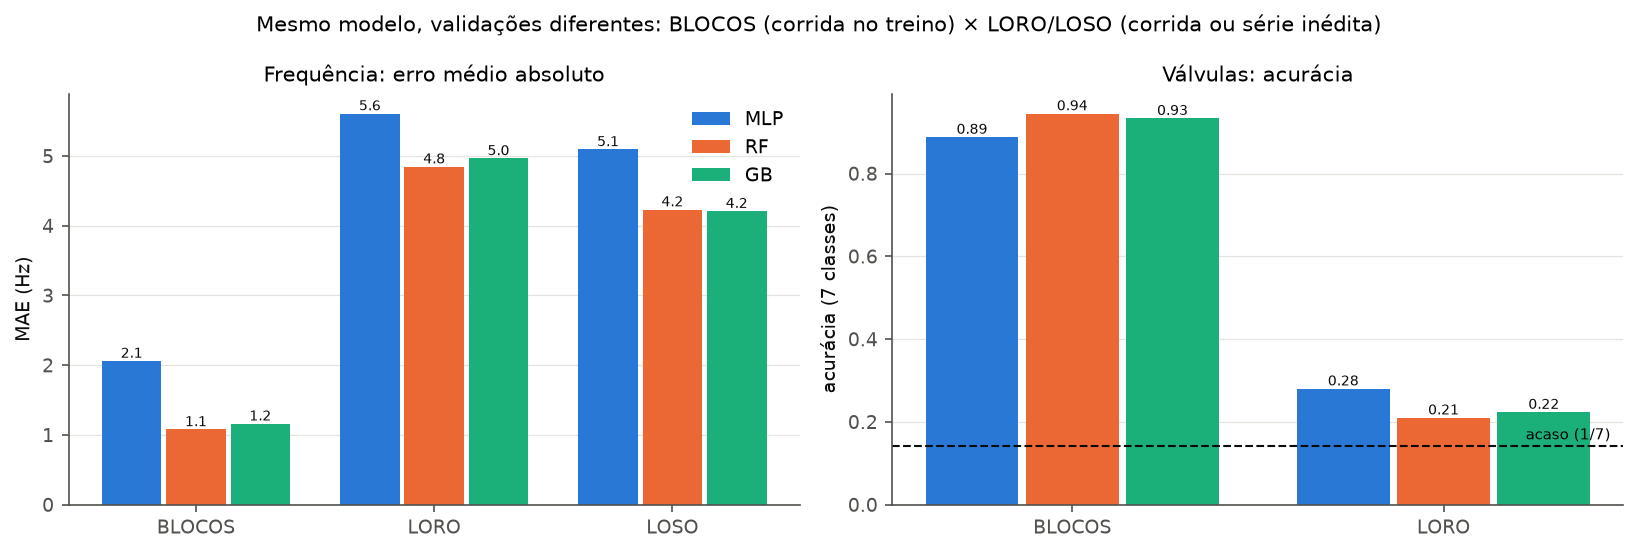
\includegraphics[width=\textwidth]{fig_blocos_vs_loro.png}
	\caption{Bomba: o mesmo modelo avaliado por validações diferentes. A frequência perde precisão, mas generaliza; as válvulas caem para perto do acaso quando a corrida sai do treino.}
	\label{fig:blocos_loro}
\end{figure}

A importância por permutação indicou que a frequência é estimada sobretudo pela energia por segundo e pelos percentis de energia, isto é, pelo nível de emissão contínua, que cresce com a rotação; para as válvulas, dominam descritores de forma e continuidade (frequência média, fração MAXDUR, duração e contagens), que, pelo resultado em LORO, identificam a corrida. Uma verificação não supervisionada confirmou o quadro: o \textit{k}-means com \(k = 8\) teve índice de Rand ajustado \cite{hubert1985} de 0,31 contra a frequência e de 0,10 contra as válvulas, e, com \(k = 56\), de 0,47 contra as corridas. Variar o tamanho da janela (2\,s) ou dispensar o corte comum de limiar não alterou as conclusões.

\paragraph{Validação interna da MLP.} A parada antecipada usa janelas sorteadas do treino, que têm vizinhas da mesma corrida no treino efetivo. Na classificação das válvulas, a validação interna indicou cerca de 90\,\% de acurácia nos folds LORO, enquanto o teste deu 18\,\%. Isso não contamina o teste, mas significa que a parada antecipada escolhe a época que melhor reconhece corridas já vistas; uma validação interna por corrida inteira seria mais coerente.

\subsection{CWRU: limiar do extrator e física do defeito}
\label{subsec:res_cwru}

A Figura~\ref{fig:sinais} mostra trechos das quatro condições com os \textit{hits} detectados. Na pista interna, com RMS de 0,58\,\(g\), o sinal fica acima do limiar fixo quase o tempo todo, e os impactos se fundem: numa gravação, 95\,\% dos \textit{hits} foram truncados pela duração máxima. É o mesmo regime de emissão contínua observado na bomba. Com o limiar flutuante, a fração truncada caiu para no máximo 1\,\% em todas as gravações, e a ordem do intervalo entre \textit{hits} passou a coincidir com as frequências de defeito: 3,60 na pista externa (BPFO = 3,58) e 5,27 na interna (BPFI = 5,42), com o pequeno desvio compatível com impactos perdidos fora da zona de carga (Figura~\ref{fig:ordem_ihi}). A esfera ficou dispersa, o que concorda com a dificuldade conhecida desses defeitos na base \cite{smith2015}. Esse descritor é obtido sem FFT, apenas com os instantes dos \textit{hits}.

\begin{figure}[!htbp]
	\centering
	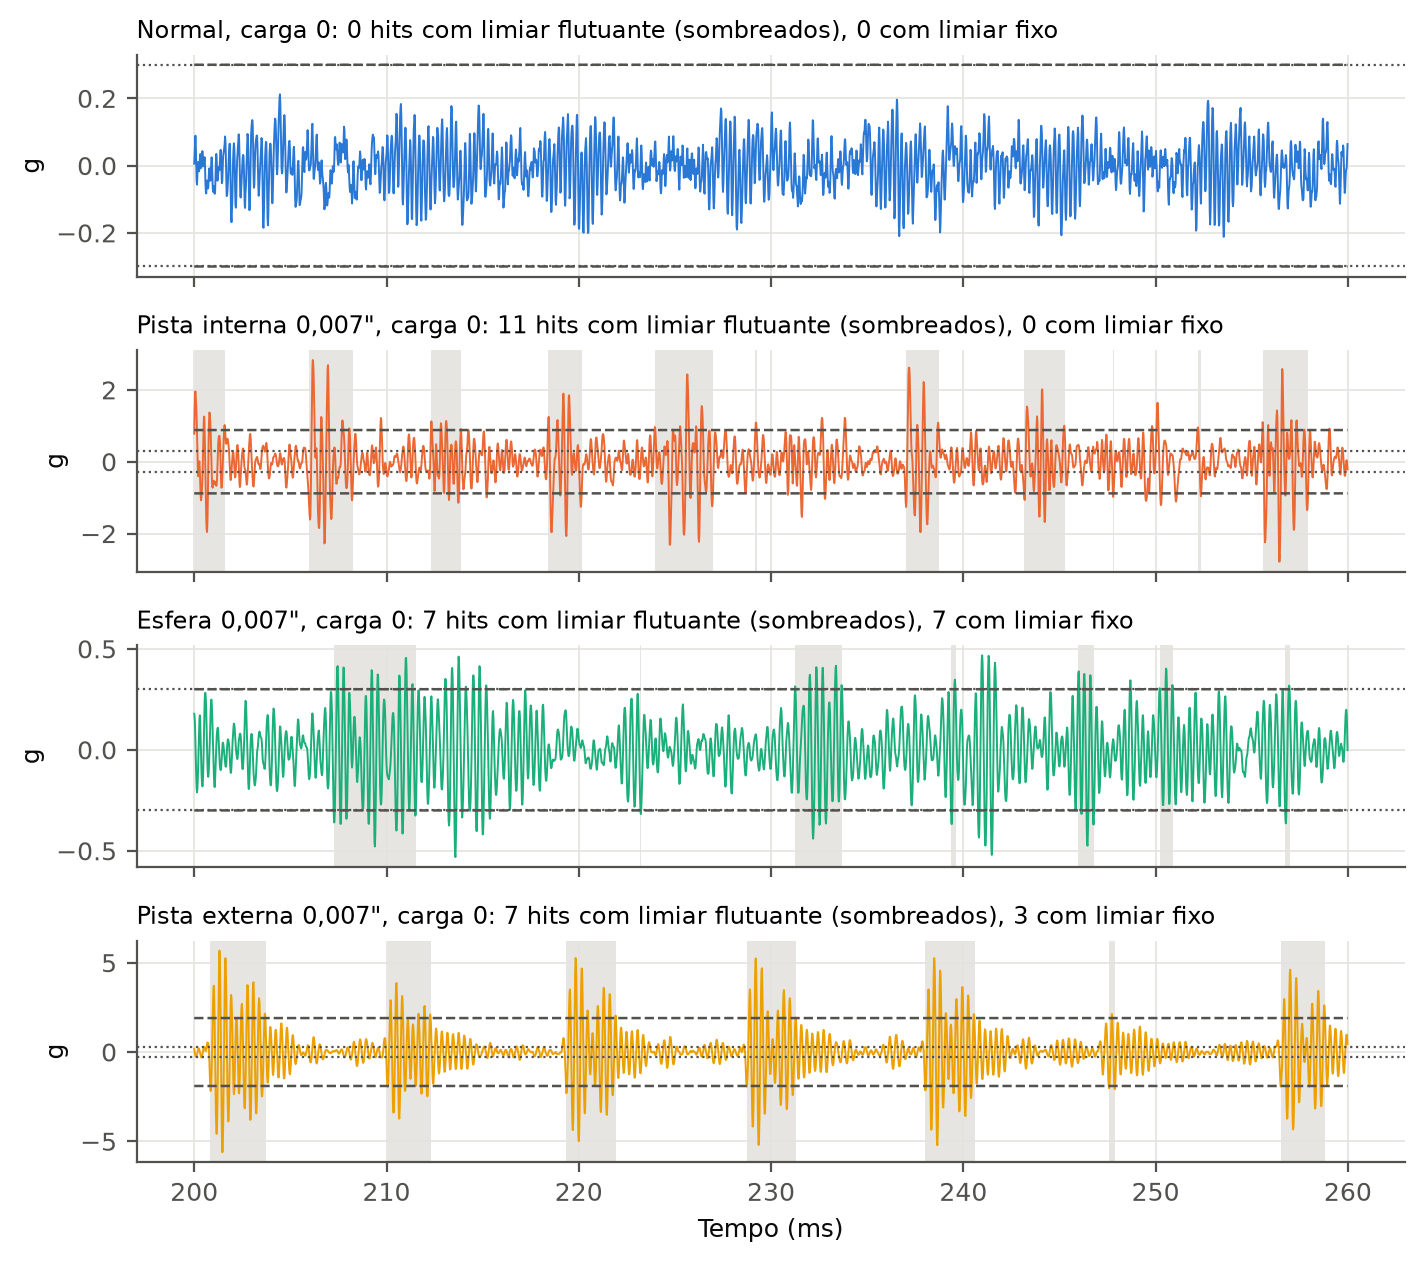
\includegraphics[width=0.78\textwidth]{fig_sinais_hits.png}
	\caption{CWRU: trechos de 60\,ms das quatro condições (carga 0, diâmetro de 0,007~polegada). Linhas pontilhadas: limiar fixo de 0,3\,\(g\); tracejadas: limiar flutuante. Áreas sombreadas: \textit{hits} detectados com o limiar flutuante.}
	\label{fig:sinais}
\end{figure}

\begin{figure}[!htbp]
	\centering
	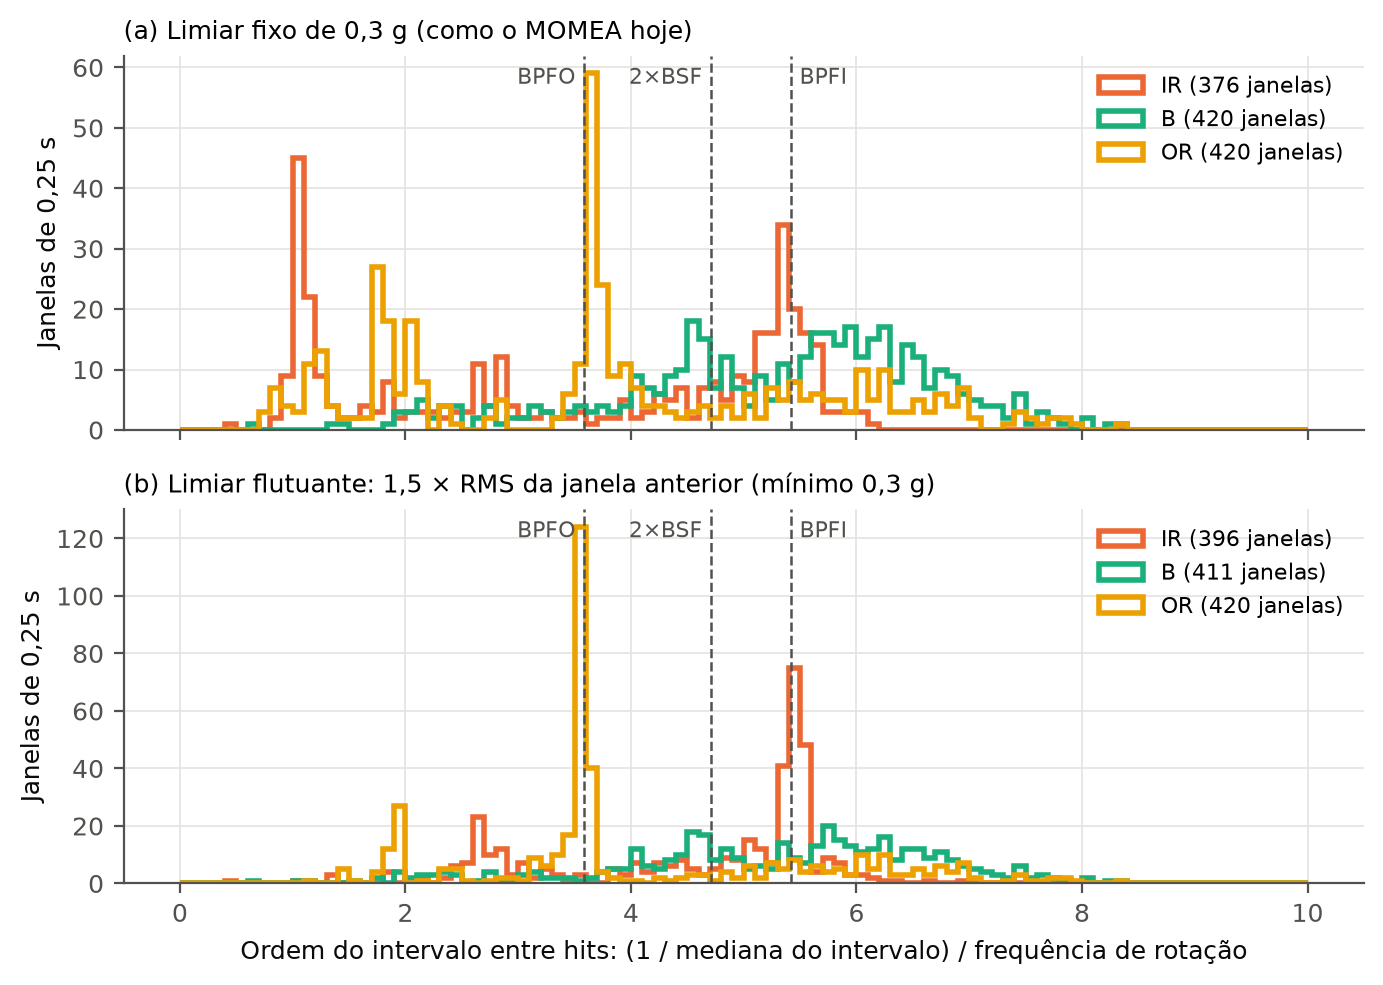
\includegraphics[width=0.8\textwidth]{fig_ordem_ihi.png}
	\caption{CWRU: ordem do intervalo entre \textit{hits} por janela, (a) com limiar fixo e (b) com limiar flutuante. Linhas tracejadas: frequências de defeito teóricas em múltiplos da rotação.}
	\label{fig:ordem_ihi}
\end{figure}

\subsection{CWRU: a acurácia depende da validação}
\label{subsec:res_cwru_val}

Com janelas sorteadas, todos os grupos de descritores chegaram a 87--92\,\% em quatro classes, e deixar uma carga de fora quase não mudou o quadro (82--90\,\%), porque o teste ainda contém os mesmos rolamentos físicos (Tabela~\ref{tab:cwru}, Figura~\ref{fig:acuracia}). Com o diâmetro inteiro fora do treino, a MLP caiu para perto do acaso com descritores de amplitude: 21\,\% com os clássicos e 25\,\% com os \textit{hits} de limiar fixo. Os \textit{hits} com limiar flutuante sustentaram 46\,\% (53\,\% com RF), e o envelope, que mede diretamente as frequências de defeito, 63\,\%. Juntar todos os descritores não ajudou a MLP (41\,\%): os descritores de amplitude dominam o ajuste e não se transferem entre rolamentos, porque a severidade não é monotônica com o diâmetro. A máquina sã é sempre reconhecida; os erros estão em distinguir os defeitos entre si, sobretudo a esfera.

\begin{table}[!htbp]
	\centering
	\small
	\caption{CWRU: acurácia (\%) por janela em quatro classes (entre parênteses, por gravação, com voto majoritário). Acaso: 25\,\%.}
	\label{tab:cwru}
	\begin{tabular}{llccc}
		\toprule
		\textbf{Descritores} & \textbf{Modelo} & \textbf{Sorteada} & \textbf{Carga de fora} & \textbf{Diâmetro de fora} \\
		\midrule
		Clássicos & MLP & 86,8 (87,5) & 82,5 (82,5) & 21,2 (25,6) \\
		 & RF & 89,5 (92,5) & 86,4 (87,5) & 28,4 (28,2) \\
		Envelope & MLP & 86,5 (90,0) & 85,2 (90,0) & \textbf{62,9} (66,7) \\
		 & RF & 87,4 (90,0) & 85,8 (90,0) & 58,0 (59,0) \\
		\textit{Hits}, limiar fixo & MLP & 87,1 (90,0) & 82,3 (85,0) & 24,6 (20,5) \\
		 & RF & 88,7 (95,0) & 84,4 (80,0) & 35,3 (38,5) \\
		\textit{Hits}, limiar flutuante & MLP & 89,2 (92,5) & 82,1 (82,5) & 45,7 (43,6) \\
		 & RF & 90,5 (92,5) & 87,9 (90,0) & 53,3 (51,3) \\
		Todos (flutuante) & MLP & 89,8 (90,0) & 88,4 (87,5) & 41,4 (38,5) \\
		 & RF & 91,9 (90,0) & 89,6 (87,5) & 54,3 (51,3) \\
		\bottomrule
	\end{tabular}
\end{table}

\begin{figure}[!htbp]
	\centering
	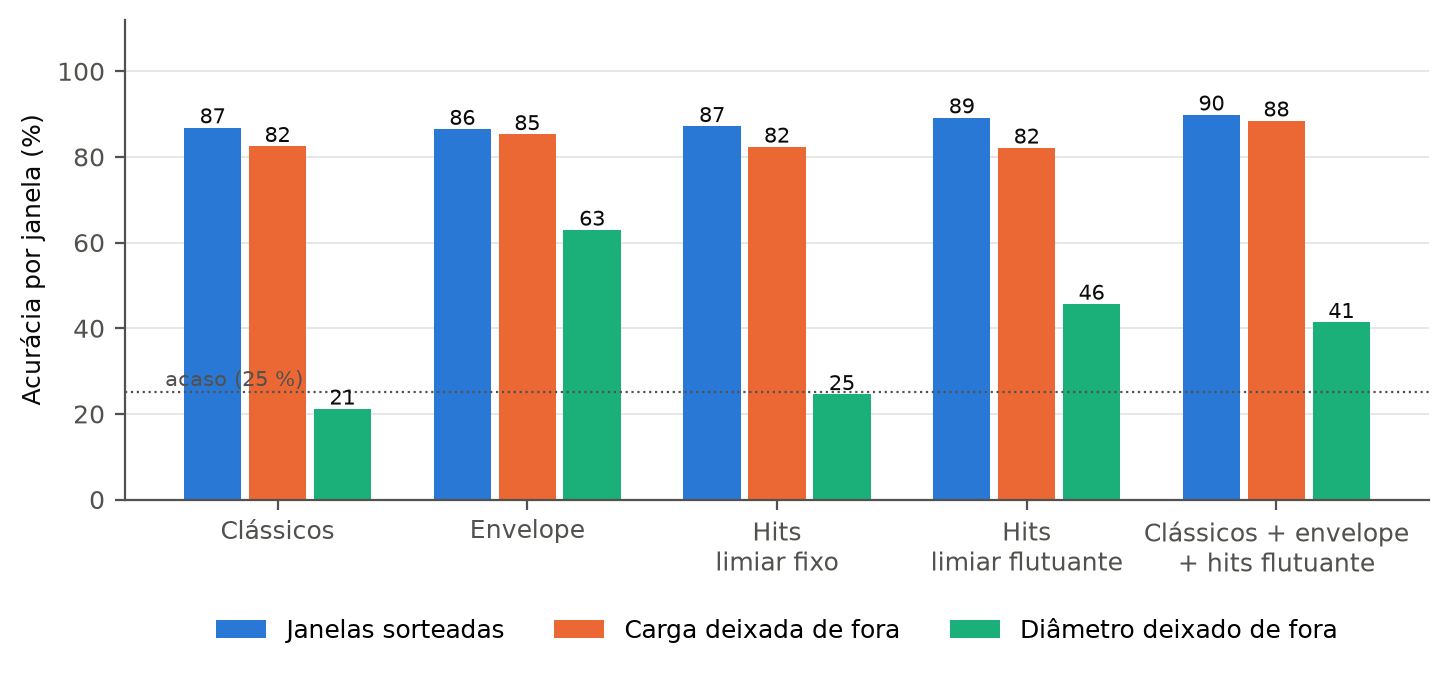
\includegraphics[width=0.72\textwidth]{fig_acuracia_validacoes.png}
	\caption{CWRU: acurácia por janela da MLP em quatro classes, por grupo de descritores e validação. A linha pontilhada marca o acaso (25\,\%).}
	\label{fig:acuracia}
\end{figure}

\subsection{Inferência embarcada}
\label{subsec:res_embarcado}

\paragraph{Fidelidade numérica (V0 a V2).} A rede reconstruída a partir dos pesos exportados reproduziu o scikit-learn com diferença máxima de \(7\times10^{-13}\)\,Hz; em C, o float32 ficou a no máximo \(2{,}5\times10^{-4}\)\,Hz, e o int8 reproduziu bit a bit os acumuladores e as classes da emulação nas 3\,540 janelas. O efeito da própria quantização (int8 contra float32) foi pequeno e centrado: \(|\Delta f|\) médio de 0,81\,Hz, com 95\,\% das janelas abaixo de 2,3\,Hz, mesmo nível de frequência em 96,6\,\% e mesma classe de válvulas em 98,2\,\% (Figura~\ref{fig:quantizacao}, Tabela~\ref{tab:fidelidade}). Partindo dos registros brutos, a cadeia completa em C com percentis exatos devolveu a mesma classe e o mesmo nível que o Python em 100\,\% das janelas; com histogramas, em 97,4 e 96,2\,\%. Na CWRU, a MLP int8 concordou com a de ponto flutuante em 98,4 a 100\,\% das janelas da validação por carga, com variação de acurácia de no máximo 0,5 ponto percentual.

\begin{figure}[!htbp]
	\centering
	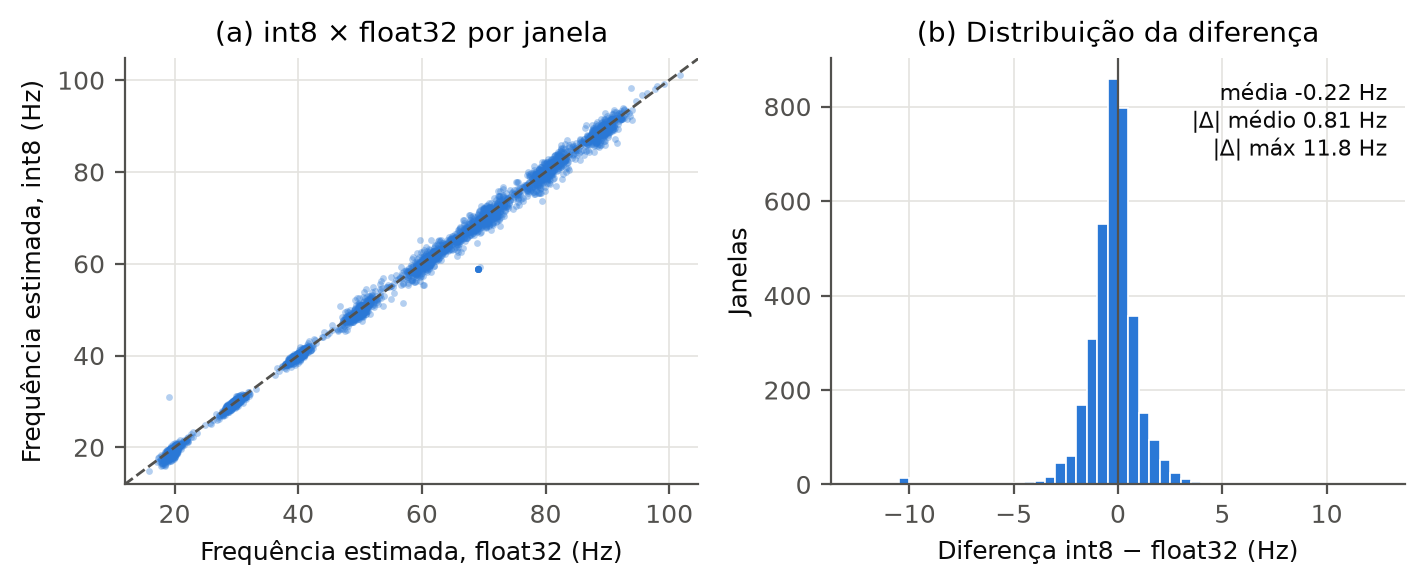
\includegraphics[width=0.8\textwidth]{fig_quantizacao.png}
	\caption{Efeito da quantização int8 sobre a frequência estimada nas 3\,540 janelas da bomba: (a) estimativa int8 contra float32, com a reta identidade tracejada; (b) distribuição da diferença.}
	\label{fig:quantizacao}
\end{figure}

\begin{table}[!htbp]
	\centering
	\small
	\caption{Concordância entre implementações (3\,540 janelas da bomba). ``Nível'' é a frequência arredondada a 10\,Hz.}
	\label{tab:fidelidade}
	\begin{tabular}{L{0.45\textwidth}ccc}
		\toprule
		\textbf{Comparação} & \textbf{Classe igual} & \textbf{Nível igual} & \textbf{\(|\Delta f|\) máx.} \\
		\midrule
		C float32 \(\times\) scikit-learn & 100\,\% & 100\,\% & \(2{,}5\times10^{-4}\)\,Hz \\
		C int8 \(\times\) emulação int8 (Python) & 100\,\% & 100\,\% & 0 (bit a bit) \\
		int8 \(\times\) float32 (efeito da quantização) & 98,2\,\% & 96,6\,\% & 11,8\,Hz \\
		Cadeia em C, percentis exatos \(\times\) Python & 100\,\% & 100\,\% & 1,2\,Hz \\
		Cadeia em C, histograma \(\times\) Python & 97,4\,\% & 96,2\,\% & 6,4\,Hz \\
		\bottomrule
	\end{tabular}
\end{table}

\paragraph{Lógica dedicada (V3 e V4).} A simulação C e a cossimulação C/RTL do núcleo HLS, com 256 janelas, terminaram sem divergência nos acumuladores ou na classe. A latência das duas redes foi de cerca de 11\,391 ciclos, ou 114\,\(\mu\)s a 100\,MHz. Após posicionamento e roteamento fora de contexto, o IP ocupou 656 LUTs (3,2\,\% do XC7A35T), 682 \textit{flip-flops} (1,6\,\%), 14 DSPs (15,6\,\%) e 3,5 blocos de BRAM (7,0\,\%), com período mínimo de 6,84\,ns.

\paragraph{MicroBlaze (V5).} As seis simulações RTL terminaram com a mesma sequência de resultados da execução no computador. A Tabela~\ref{tab:ciclos} resume os ciclos medidos. \mbParagrafoMlp

\begin{table}[!htbp]
	\centering
	\small
	\caption{Ciclos medidos na simulação RTL da MicroBlaze (100\,MHz, memória local, sem caches).}
	\label{tab:ciclos}
	\begin{tabular}{lrr}
		\toprule
		\textbf{Etapa} & \textbf{Sem FPU} & \textbf{Com FPU} \\
		\midrule
		MLP float32, duas redes & \mbMlpFloatSoft & \mbMlpFloatFpu \\
		Núcleo int8, duas redes & \mbMlpIntSoft & \mbMlpIntFpu \\
		Inferência int8 completa (\(\mu\)s) & \mbMlpIntSoftUs & \mbMlpIntFpuUs \\
		Por \textit{hit}, modo exato & \mbHitSoft & \mbHitFpu \\
		Fechar a janela, modo exato & \mbFecharSoft & \mbFecharFpu \\
		Fechar a janela, modo histograma & \mbFecharHistSoft & \mbFecharHistFpu \\
		\bottomrule
	\end{tabular}
\end{table}

\mbParagrafoCarga{} A Figura~\ref{fig:carga} extrapola essa ocupação em função da taxa de \textit{hits}. Os ciclos medidos representam o melhor caso do código, sem caches, interrupções nem pilha de rede concorrendo.

\begin{figure}[!htbp]
	\centering
	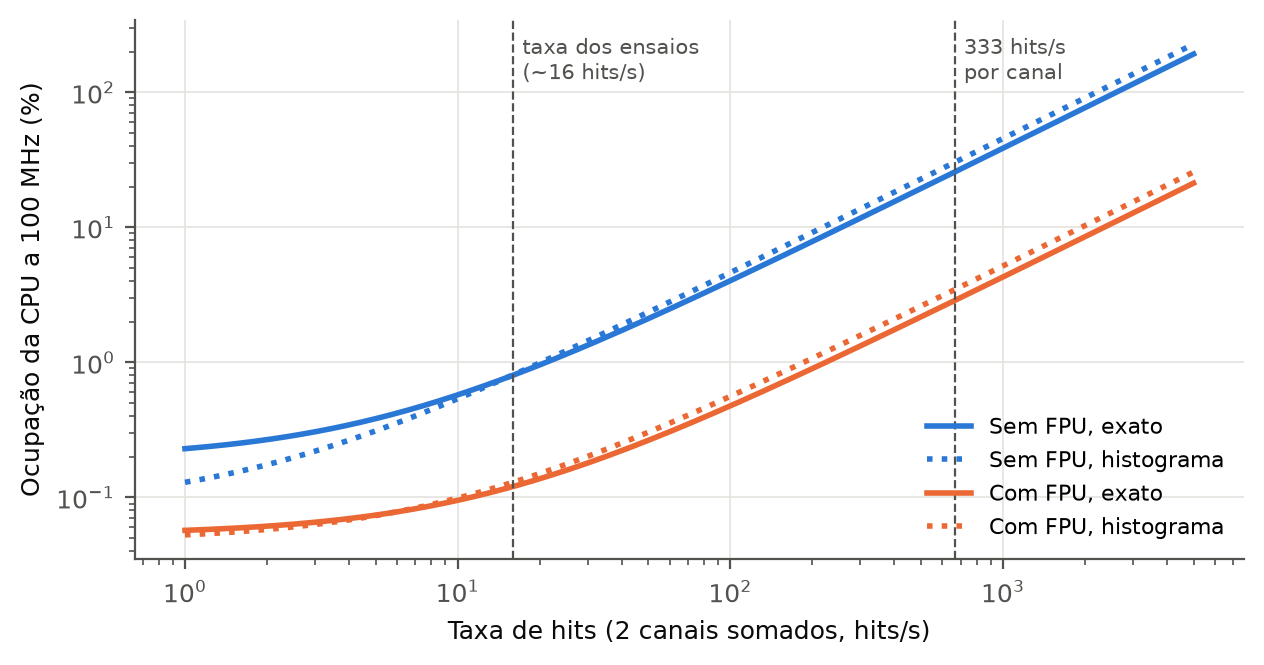
\includegraphics[width=0.75\textwidth]{fig_carga_cpu.png}
	\caption{Ocupação da CPU da MicroBlaze a 100\,MHz pela cadeia embarcada em função da taxa de \textit{hits}, extrapolada dos ciclos medidos. As linhas verticais marcam a taxa dos ensaios da bomba e a maior taxa sustentada em ensaio elétrico.}
	\label{fig:carga}
\end{figure}

% =======================================================================================================
\section{Discussão}
\label{sec:discussao}

\paragraph{A validação precisa separar as unidades físicas.} Na bomba e na CWRU, as validações que mantêm a unidade física (a corrida ou o rolamento) no treino e no teste deram 82--95\,\% com qualquer modelo ou grupo de descritores. Quando a unidade saiu do treino, as válvulas da bomba caíram para 21--28\,\% e os descritores de amplitude da CWRU para perto do acaso. A diferença entre os dois casos é instrutiva: na CWRU sabe-se que os defeitos são reais e localizados, de modo que a queda não pode ser atribuída à ausência de efeito físico, mas à pouca diversidade de unidades (nove rolamentos com defeito). Na bomba, o resultado não prova que as válvulas não tenham assinatura de EA; ele mostra que, com uma corrida por condição e as séries em blocos contínuos, o efeito da válvula está confundido com o dia, o horário e o limiar. Comparações com outros trabalhos na base CWRU só fazem sentido sob o mesmo esquema de validação \cite{rauber2021,hendriks2022}.

\paragraph{MLP, RF e GB.} Os três modelos tiveram desempenho semelhante na bomba; na CWRU, a RF foi um pouco melhor fora da amostra com \textit{hits} e com todos os descritores, e a MLP com o envelope. Isso concorda com a literatura sobre dados tabulares \cite{fernandezdelgado2014,grinsztajn2022,shwartzziv2022} e indica que o limite está nos dados e nos descritores, e não no modelo. A escolha da MLP para a borda justifica-se pela implementação: uma sequência fixa de 8\,960 multiplicações-acumulações, sem desvios dependentes dos dados, que quantiza em int8 com perda desprezível e cabe tanto na MicroBlaze quanto em 3\,\% das LUTs do FPGA.

\paragraph{O extrator condiciona os descritores.} Com limiar fixo, a emissão contínua funde os \textit{hits} e os trunca pela duração máxima; na bomba, isso somou-se à saturação do conversor a partir de 40\,Hz e à cadência imposta pelo rearme, de modo que amplitude, energia e taxa de \textit{hits} perderam informação justamente onde as condições mais se confundem. Na CWRU, o limiar flutuante eliminou a truncagem, recuperou a periodicidade do defeito sem FFT e quase dobrou a acurácia fora da amostra, ficando a meio caminho do envelope por uma fração do custo: o envelope exige filtragem, transformada de Hilbert e FFTs de 16\,384 pontos por janela, inviáveis na MicroBlaze sem FPU, enquanto os descritores de \textit{hits} custam \mbHitFpu{} ciclos por \textit{hit} com FPU.

\paragraph{Embarcado.} Para uma decisão a cada 5\,s, as duas rotas sobram. \mbParagrafoRota{} O IP HLS é \mbFatorHls{} vezes mais rápido que a MicroBlaze sem FPU e libera o processador, ao custo de 14 DSPs e 3,5 blocos de BRAM; ele se justificaria para modelos maiores ou taxas de \textit{hits} muito altas. A parte cara da cadeia não é a rede, mas o processamento por \textit{hit}, dominado pelos logaritmos. A simulação garante a fidelidade e mede o custo, mas não cobre a integração com o projeto atual do MOMEA, o tempo de parede com a pilha de rede, a base de tempo das janelas no relógio local nem o comportamento elétrico do \textit{front-end}.

\paragraph{Limitações.} (i) A bomba não tem repetições: a variabilidade entre repetições não pôde ser estimada, e BLOCOS é otimista por construção. (ii) Válvulas, dia, horário e limiar estão confundidos. (iii) A saturação acima de 40\,Hz e a cadência do rearme limitam os descritores da bomba. (iv) Na CWRU, os sinais são de vibração a 48\,kHz, e as conclusões não se transferem diretamente para EA de alta frequência; o fator do limiar flutuante foi escolhido com os rótulos, e há só três partições por diâmetro. (v) Os hiperparâmetros são fixos, e os resultados são linhas de base.

\paragraph{Recomendações.} Para o próximo ensaio: repetir cada condição duas ou três vezes em ordem aleatorizada; manter ganho e limiar fixos e reduzir o ganho para evitar a saturação; complementar os \textit{hits} com descritores de nível (RMS, energia por intervalo, bandas espectrais) \cite{derakhshan1991}; e reservar uma campanha inteira como teste final. Para o MOMEA: implementar um limiar flutuante na lógica e o carimbo de tempo de \textit{hardware}, que viabiliza os descritores de periodicidade; confirmar no HDL o limite do bloqueio re-armável; e usar, na parada antecipada da MLP, uma validação interna por corrida inteira.

% =======================================================================================================
\section{Conclusões}
\label{sec:conclusoes}

Redes MLP sobre descritores de \textit{hits} extraídos no FPGA do MOMEA estimaram a frequência do motor de uma bomba com MAE de 4,2 a 5,6\,Hz em corridas e sessões não vistas, com desempenho semelhante ao de florestas aleatórias e \textit{gradient boosting}. A configuração das válvulas só foi reconhecida quando a própria corrida estava no treino. Na base CWRU, o mesmo fluxo reproduziu o padrão: 87--92\,\% com janelas sorteadas e 21--63\,\% com rolamentos nunca vistos, dependendo dos descritores; os \textit{hits} com limiar flutuante recuperaram a periodicidade dos defeitos e ficaram a meio caminho entre os descritores de amplitude e o envelope. A cadeia de descritores e as MLPs int8 foram levadas ao Artix-7 e verificadas por simulação até o nível RTL do processador, reproduzindo o modelo de referência em 100\,\% das janelas, com 114\,\(\mu\)s por inferência no IP dedicado e menos de \mbCargaEnsaioMax\,\% de CPU na MicroBlaze.

A MLP é, portanto, viável na borda; o que limita a generalização são os dados e o extrator. A diferença entre validações é o principal resultado metodológico: em dados de EA com uma unidade física por condição, dividir \textit{hits} ou janelas ao acaso superestima a capacidade de classificação. Ensaios com repetições aleatorizadas, ganho e limiar fixos, limiar flutuante no extrator e descritores contínuos são os próximos passos; os modelos resultantes entram no mesmo fluxo embarcado sem mudanças no código.

% =======================================================================================================
{\small
\begin{thebibliography}{99}
\setlength{\itemsep}{1pt}

	\bibitem[Alfayez et al.(2005)]{alfayez2005}
	ALFAYEZ, L.; MBA, D.; DYSON, G.
	\newblock The application of acoustic emission for detecting incipient cavitation and the best efficiency point of a 60 kW centrifugal pump: case study.
	\newblock \emph{NDT \& E International}, v. 38, n. 5, p. 354--358, 2005.
	\newblock DOI: \href{https://doi.org/10.1016/j.ndteint.2004.10.002}{10.1016/j.ndteint.2004.10.002}.

	\bibitem[AMD(2022a)]{amd_ug1399}
	AMD.
	\newblock \emph{Vitis High-Level Synthesis User Guide (UG1399)}, v2022.2.
	\newblock San Jose: Advanced Micro Devices, 2022.

	\bibitem[AMD(2022b)]{amd_ug984}
	AMD.
	\newblock \emph{MicroBlaze Processor Reference Guide (UG984)}, v2022.2.
	\newblock San Jose: Advanced Micro Devices, 2022.

	\bibitem[AMD(2022c)]{amd_ug900}
	AMD.
	\newblock \emph{Vivado Design Suite User Guide: Logic Simulation (UG900)}, v2022.2.
	\newblock San Jose: Advanced Micro Devices, 2022.

	\bibitem[Amini et al.(2022)]{amini2022}
	AMINI, A.; PACOT, O.; VOIDE, D.; HASMATUCHI, V.; RODUIT, P.; MÜNCH-ALLIGNÉ, C.
	\newblock Development of a novel cavitation monitoring system for hydro turbines based on machine learning algorithms.
	\newblock \emph{IOP Conference Series: Earth and Environmental Science}, v. 1079, art. 012015, 2022.
	\newblock DOI: \href{https://doi.org/10.1088/1755-1315/1079/1/012015}{10.1088/1755-1315/1079/1/012015}.

	\bibitem[Breiman(2001)]{breiman2001}
	BREIMAN, L.
	\newblock Random forests.
	\newblock \emph{Machine Learning}, v. 45, n. 1, p. 5--32, 2001.
	\newblock DOI: \href{https://doi.org/10.1023/A:1010933404324}{10.1023/A:1010933404324}.

	\bibitem[Brennen(1995)]{brennen1995}
	BRENNEN, C. E.
	\newblock \emph{Cavitation and Bubble Dynamics}.
	\newblock New York: Oxford University Press, 1995.

	\bibitem[CWRU(s.d.)]{cwru}
	CASE WESTERN RESERVE UNIVERSITY.
	\newblock \emph{Bearing Data Center}: 48k Drive End Bearing Fault Data; Normal Baseline Data.
	\newblock Disponível em: \url{https://engineering.case.edu/bearingdatacenter}. Acesso em: 10 nov. 2026.

	\bibitem[Chen e Guestrin(2016)]{chen2016}
	CHEN, T.; GUESTRIN, C.
	\newblock XGBoost: a scalable tree boosting system.
	\newblock In: ACM SIGKDD INTERNATIONAL CONFERENCE ON KNOWLEDGE DISCOVERY AND DATA MINING, 22., 2016, San Francisco. \emph{Proceedings} [...]. New York: ACM, 2016. p. 785--794.
	\newblock DOI: \href{https://doi.org/10.1145/2939672.2939785}{10.1145/2939672.2939785}.

	\bibitem[Derakhshan et al.(1991)]{derakhshan1991}
	DERAKHSHAN, O.; HOUGHTON, J. R.; JONES, R. K.; MARCH, P. A.
	\newblock Cavitation monitoring of hydroturbines with RMS acoustic emission measurement.
	\newblock In: \emph{ASTM Special Technical Publication 1077}.
	\newblock Philadelphia: ASTM, 1991. p. 305--315.
	\newblock DOI: \href{https://doi.org/10.1520/STP19102S}{10.1520/STP19102S}.

	\bibitem[Duarte et al.(2018)]{duarte2018}
	DUARTE, J. et al.
	\newblock Fast inference of deep neural networks in FPGAs for particle physics.
	\newblock \emph{Journal of Instrumentation}, v. 13, n. 7, P07027, 2018.
	\newblock DOI: \href{https://doi.org/10.1088/1748-0221/13/07/P07027}{10.1088/1748-0221/13/07/P07027}.

	\bibitem[Escaler et al.(2006)]{escaler2006}
	ESCALER, X.; EGUSQUIZA, E.; FARHAT, M.; AVELLAN, F.; COUSSIRAT, M.
	\newblock Detection of cavitation in hydraulic turbines.
	\newblock \emph{Mechanical Systems and Signal Processing}, v. 20, p. 983--1007, 2006.
	\newblock DOI: \href{https://doi.org/10.1016/j.ymssp.2004.08.006}{10.1016/j.ymssp.2004.08.006}.

	\bibitem[Fernández-Delgado et al.(2014)]{fernandezdelgado2014}
	FERNÁNDEZ-DELGADO, M.; CERNADAS, E.; BARRO, S.; AMORIM, D.
	\newblock Do we need hundreds of classifiers to solve real world classification problems?
	\newblock \emph{Journal of Machine Learning Research}, v. 15, p. 3133--3181, 2014.

	\bibitem[Friedman(2001)]{friedman2001}
	FRIEDMAN, J. H.
	\newblock Greedy function approximation: a gradient boosting machine.
	\newblock \emph{The Annals of Statistics}, v. 29, n. 5, p. 1189--1232, 2001.
	\newblock DOI: \href{https://doi.org/10.1214/aos/1013203451}{10.1214/aos/1013203451}.

	\bibitem[Goldberg(1991)]{goldberg1991}
	GOLDBERG, D.
	\newblock What every computer scientist should know about floating-point arithmetic.
	\newblock \emph{ACM Computing Surveys}, v. 23, n. 1, p. 5--48, 1991.
	\newblock DOI: \href{https://doi.org/10.1145/103162.103163}{10.1145/103162.103163}.

	\bibitem[Grinsztajn et al.(2022)]{grinsztajn2022}
	GRINSZTAJN, L.; OYALLON, E.; VAROQUAUX, G.
	\newblock Why do tree-based models still outperform deep learning on typical tabular data?
	\newblock In: \emph{Advances in Neural Information Processing Systems 35} (NeurIPS 2022), Datasets and Benchmarks Track, 2022.

	\bibitem[Grosse et al.(2022)]{grosse2022}
	GROSSE, C. U.; OHTSU, M.; AGGELIS, D. G.; SHIOTANI, T. (ed.).
	\newblock \emph{Acoustic Emission Testing: Basics for Research -- Applications in Engineering}.
	\newblock 2. ed. Cham: Springer, 2022.
	\newblock DOI: \href{https://doi.org/10.1007/978-3-030-67936-1}{10.1007/978-3-030-67936-1}.

	\bibitem[Hendriks et al.(2022)]{hendriks2022}
	HENDRIKS, J.; DUMOND, P.; KNOX, D. A.
	\newblock Towards better benchmarking using the CWRU bearing fault dataset.
	\newblock \emph{Mechanical Systems and Signal Processing}, v. 169, art. 108732, 2022.
	\newblock DOI: \href{https://doi.org/10.1016/j.ymssp.2021.108732}{10.1016/j.ymssp.2021.108732}.

	\bibitem[Hornik et al.(1989)]{hornik1989}
	HORNIK, K.; STINCHCOMBE, M.; WHITE, H.
	\newblock Multilayer feedforward networks are universal approximators.
	\newblock \emph{Neural Networks}, v. 2, n. 5, p. 359--366, 1989.

	\bibitem[Hubert e Arabie(1985)]{hubert1985}
	HUBERT, L.; ARABIE, P.
	\newblock Comparing partitions.
	\newblock \emph{Journal of Classification}, v. 2, n. 1, p. 193--218, 1985.
	\newblock DOI: \href{https://doi.org/10.1007/BF01908075}{10.1007/BF01908075}.

	\bibitem[IEEE(2019)]{ieee754}
	IEEE.
	\newblock \emph{IEEE Standard for Floating-Point Arithmetic} (IEEE Std 754-2019).
	\newblock New York: IEEE, 2019.

	\bibitem[Jacob et al.(2018)]{jacob2018}
	JACOB, B.; KLIGYS, S.; CHEN, B.; ZHU, M.; TANG, M.; HOWARD, A.; ADAM, H.; KALENICHENKO, D.
	\newblock Quantization and training of neural networks for efficient integer-arithmetic-only inference.
	\newblock In: \emph{IEEE/CVF Conference on Computer Vision and Pattern Recognition (CVPR)}, 2018. p. 2704--2713.

	\bibitem[Kang et al.(2015)]{kang2015}
	KANG, M.; KIM, J.; KIM, J.-M.
	\newblock An FPGA-based multicore system for real-time bearing fault diagnosis using ultrasampling rate AE signals.
	\newblock \emph{IEEE Transactions on Industrial Electronics}, v. 62, n. 4, p. 2319--2329, 2015.
	\newblock DOI: \href{https://doi.org/10.1109/TIE.2014.2361317}{10.1109/TIE.2014.2361317}.

	\bibitem[Kaufman et al.(2012)]{kaufman2012}
	KAUFMAN, S.; ROSSET, S.; PERLICH, C.; STITELMAN, O.
	\newblock Leakage in data mining: formulation, detection, and avoidance.
	\newblock \emph{ACM Transactions on Knowledge Discovery from Data}, v. 6, n. 4, art. 15, 2012.
	\newblock DOI: \href{https://doi.org/10.1145/2382577.2382579}{10.1145/2382577.2382579}.

	\bibitem[Ke et al.(2017)]{ke2017}
	KE, G.; MENG, Q.; FINLEY, T.; WANG, T.; CHEN, W.; MA, W.; YE, Q.; LIU, T.-Y.
	\newblock LightGBM: a highly efficient gradient boosting decision tree.
	\newblock In: \emph{Advances in Neural Information Processing Systems 30} (NIPS 2017), 2017. p. 3146--3154.

	\bibitem[Kingma e Ba(2015)]{kingma2015}
	KINGMA, D. P.; BA, J.
	\newblock Adam: a method for stochastic optimization.
	\newblock In: INTERNATIONAL CONFERENCE ON LEARNING REPRESENTATIONS, 3., 2015, San Diego. \emph{Proceedings} [...]. 2015.
	\newblock Disponível em: \href{https://arxiv.org/abs/1412.6980}{arXiv:1412.6980}.

	\bibitem[Krishnamoorthi(2018)]{krishnamoorthi2018}
	KRISHNAMOORTHI, R.
	\newblock Quantizing deep convolutional networks for efficient inference: a whitepaper.
	\newblock arXiv:1806.08342, 2018.

	\bibitem[Lei et al.(2020)]{lei2020}
	LEI, Y.; YANG, B.; JIANG, X.; JIA, F.; LI, N.; NANDI, A. K.
	\newblock Applications of machine learning to machine fault diagnosis: a review and roadmap.
	\newblock \emph{Mechanical Systems and Signal Processing}, v. 138, art. 106587, 2020.
	\newblock DOI: \href{https://doi.org/10.1016/j.ymssp.2019.106587}{10.1016/j.ymssp.2019.106587}.

	\bibitem[Liu et al.(2023)]{liu2023}
	LIU, X.; MOU, J.; XU, X.; QIU, Z.; DONG, B.
	\newblock A review of pump cavitation fault detection methods based on different signals.
	\newblock \emph{Processes}, v. 11, n. 7, art. 2007, 2023.
	\newblock DOI: \href{https://doi.org/10.3390/pr11072007}{10.3390/pr11072007}.

	\bibitem[Mba(2006)]{mba2006}
	MBA, D.
	\newblock Development of acoustic emission technology for condition monitoring and diagnosis of rotating machines: bearings, pumps, gearboxes, engines, and rotating structures.
	\newblock \emph{The Shock and Vibration Digest}, v. 38, n. 1, p. 3--16, 2006.
	\newblock DOI: \href{https://doi.org/10.1177/0583102405059054}{10.1177/0583102405059054}.

	\bibitem[Mousmoulis et al.(2019)]{mousmoulis2019}
	MOUSMOULIS, G.; KARLSEN-DAVIES, N.; AGGIDIS, G.; ANAGNOSTOPOULOS, I.; PAPANTONIS, D.
	\newblock Experimental analysis of cavitation in a centrifugal pump using acoustic emission, vibration measurements and flow visualization.
	\newblock \emph{European Journal of Mechanics -- B/Fluids}, v. 75, p. 300--311, 2019.
	\newblock DOI: \href{https://doi.org/10.1016/j.euromechflu.2018.10.015}{10.1016/j.euromechflu.2018.10.015}.

	\bibitem[Nagel et al.(2021)]{nagel2021}
	NAGEL, M.; FOURNARAKIS, M.; AMJAD, R. A.; BONDARENKO, Y.; VAN BAALEN, M.; BLANKEVOORT, T.
	\newblock A white paper on neural network quantization.
	\newblock arXiv:2106.08295, 2021.

	\bibitem[Neill et al.(1997)]{neill1997}
	NEILL, G. D.; REUBEN, R. L.; SANDFORD, P. M.; BROWN, E. R.; STEEL, J. A.
	\newblock Detection of incipient cavitation in pumps using acoustic emission.
	\newblock \emph{Proceedings of the Institution of Mechanical Engineers, Part E: Journal of Process Mechanical Engineering}, v. 211, n. 4, p. 267--277, 1997.
	\newblock DOI: \href{https://doi.org/10.1243/0954408971529737}{10.1243/0954408971529737}.

	\bibitem[Ohno e Ohtsu(2010)]{ohno2010}
	OHNO, K.; OHTSU, M.
	\newblock Crack classification in concrete based on acoustic emission.
	\newblock \emph{Construction and Building Materials}, v. 24, n. 12, p. 2339--2346, 2010.
	\newblock DOI: \href{https://doi.org/10.1016/j.conbuildmat.2010.05.004}{10.1016/j.conbuildmat.2010.05.004}.

	\bibitem[Pedregosa et al.(2011)]{pedregosa2011}
	PEDREGOSA, F. et al.
	\newblock Scikit-learn: machine learning in Python.
	\newblock \emph{Journal of Machine Learning Research}, v. 12, p. 2825--2830, 2011.

	\bibitem[Piñal-Moctezuma et al.(2019)]{pinal2019}
	PIÑAL-MOCTEZUMA, F.; DELGADO-PRIETO, M.; ROMERAL-MARTÍNEZ, L.
	\newblock Performance analysis of acoustic emission hit detection methods using time features.
	\newblock \emph{IEEE Access}, v. 7, p. 71119--71130, 2019.
	\newblock DOI: \href{https://doi.org/10.1109/ACCESS.2019.2919224}{10.1109/ACCESS.2019.2919224}.

	\bibitem[Prechelt(1998)]{prechelt1998}
	PRECHELT, L.
	\newblock Early stopping -- but when?
	\newblock In: ORR, G. B.; MÜLLER, K.-R. (ed.). \emph{Neural Networks: Tricks of the Trade}.
	\newblock Berlin: Springer, 1998. (Lecture Notes in Computer Science, v. 1524). p. 55--69.

	\bibitem[Randall e Antoni(2011)]{randall2011}
	RANDALL, R. B.; ANTONI, J.
	\newblock Rolling element bearing diagnostics---a tutorial.
	\newblock \emph{Mechanical Systems and Signal Processing}, v. 25, n. 2, p. 485--520, 2011.
	\newblock DOI: \href{https://doi.org/10.1016/j.ymssp.2010.07.017}{10.1016/j.ymssp.2010.07.017}.

	\bibitem[Rauber et al.(2021)]{rauber2021}
	RAUBER, T. W.; LOCA, A. L. S.; BOLDT, F. A.; RODRIGUES, A. L.; VAREJÃO, F. M.
	\newblock An experimental methodology to evaluate machine learning methods for fault diagnosis based on vibration signals.
	\newblock \emph{Expert Systems with Applications}, v. 167, art. 114022, 2021.
	\newblock DOI: \href{https://doi.org/10.1016/j.eswa.2020.114022}{10.1016/j.eswa.2020.114022}.

	\bibitem[Roberts et al.(2017)]{roberts2017}
	ROBERTS, D. R. et al.
	\newblock Cross-validation strategies for data with temporal, spatial, hierarchical, or phylogenetic structure.
	\newblock \emph{Ecography}, v. 40, n. 8, p. 913--929, 2017.
	\newblock DOI: \href{https://doi.org/10.1111/ecog.02881}{10.1111/ecog.02881}.

	\bibitem[Rumelhart et al.(1986)]{rumelhart1986}
	RUMELHART, D. E.; HINTON, G. E.; WILLIAMS, R. J.
	\newblock Learning representations by back-propagating errors.
	\newblock \emph{Nature}, v. 323, p. 533--536, 1986.
	\newblock DOI: \href{https://doi.org/10.1038/323533a0}{10.1038/323533a0}.

	\bibitem[Samanta e Al-Balushi(2003)]{samanta2003}
	SAMANTA, B.; AL-BALUSHI, K. R.
	\newblock Artificial neural network based fault diagnostics of rolling element bearings using time-domain features.
	\newblock \emph{Mechanical Systems and Signal Processing}, v. 17, n. 2, p. 317--328, 2003.
	\newblock DOI: \href{https://doi.org/10.1006/mssp.2001.1462}{10.1006/mssp.2001.1462}.

	\bibitem[Shwartz-Ziv e Armon(2022)]{shwartzziv2022}
	SHWARTZ-ZIV, R.; ARMON, A.
	\newblock Tabular data: deep learning is not all you need.
	\newblock \emph{Information Fusion}, v. 81, p. 84--90, 2022.
	\newblock DOI: \href{https://doi.org/10.1016/j.inffus.2021.11.011}{10.1016/j.inffus.2021.11.011}.

	\bibitem[Smith e Randall(2015)]{smith2015}
	SMITH, W. A.; RANDALL, R. B.
	\newblock Rolling element bearing diagnostics using the Case Western Reserve University data: a benchmark study.
	\newblock \emph{Mechanical Systems and Signal Processing}, v. 64--65, p. 100--131, 2015.
	\newblock DOI: \href{https://doi.org/10.1016/j.ymssp.2015.04.021}{10.1016/j.ymssp.2015.04.021}.

	\bibitem[Unn{\th}{\'o}rsson(2013)]{unnthorsson2013}
	UNN{\TH}{\'O}RSSON, R.
	\newblock Hit detection and determination in AE bursts.
	\newblock In: SIKORSKI, W. (ed.). \emph{Acoustic Emission---Research and Applications}.
	\newblock Rijeka: IntechOpen, 2013.
	\newblock DOI: \href{https://doi.org/10.5772/54754}{10.5772/54754}.

	\bibitem[Vallen Systeme(2022)]{vallen2022}
	VALLEN SYSTEME GMBH.
	\newblock \emph{AMSY-6: System Specification}.
	\newblock Wolfratshausen: Vallen Systeme GmbH, 2022.
	\newblock Disponível em: \href{https://www.vallen.de/zdownload/pdf/AMSY-6_Spec.pdf}{especificação técnica do AMSY-6}. Acesso em: 24 jul. 2026.

	\bibitem[Varma e Simon(2006)]{varma2006}
	VARMA, S.; SIMON, R.
	\newblock Bias in error estimation when using cross-validation for model selection.
	\newblock \emph{BMC Bioinformatics}, v. 7, art. 91, 2006.
	\newblock DOI: \href{https://doi.org/10.1186/1471-2105-7-91}{10.1186/1471-2105-7-91}.

	\bibitem[Wirtz et al.(2018)]{wirtz2018}
	WIRTZ, S. F.; CUNHA, A. P. A.; LABUSCH, M.; MARZUN, G.; BARCIKOWSKI, S.; SÖFFKER, D.
	\newblock Development of a low-cost FPGA-based measurement system for real-time processing of acoustic emission data: proof of concept using control of pulsed laser ablation in liquids.
	\newblock \emph{Sensors}, v. 18, n. 6, art. 1775, 2018.
	\newblock DOI: \href{https://doi.org/10.3390/s18061775}{10.3390/s18061775}.

	\bibitem[Zhang et al.(2017)]{zhang2017}
	ZHANG, W.; PENG, G.; LI, C.; CHEN, Y.; ZHANG, Z.
	\newblock A new deep learning model for fault diagnosis with good anti-noise and domain adaptation ability on raw vibration signals.
	\newblock \emph{Sensors}, v. 17, n. 2, art. 425, 2017.
	\newblock DOI: \href{https://doi.org/10.3390/s17020425}{10.3390/s17020425}.

	\bibitem[Zhang et al.(2018)]{zhang2018}
	ZHANG, W.; LI, C.; PENG, G.; CHEN, Y.; ZHANG, Z.
	\newblock A deep convolutional neural network with new training methods for bearing fault diagnosis under noisy environment and different working load.
	\newblock \emph{Mechanical Systems and Signal Processing}, v. 100, p. 439--453, 2018.
	\newblock DOI: \href{https://doi.org/10.1016/j.ymssp.2017.06.022}{10.1016/j.ymssp.2017.06.022}.

\end{thebibliography}
}

\end{document}
